\documentclass[a4paper,10pt]{article}
\usepackage[margin=0.7in]{geometry}
\usepackage{multicol}
\usepackage{array}
\usepackage{titlesec}
\usepackage{enumitem}
\usepackage{booktabs}
\usepackage{tikz}
\usepackage{amsmath}
\usepackage{longtable}
\usetikzlibrary{positioning}

% Reduce spacing
\titlespacing*{\section}{0pt}{1ex}{0.5ex}
\titlespacing*{\subsection}{0pt}{0.5ex}{0.25ex}
\setlist{nosep,left=1em}

\renewcommand{\arraystretch}{1.1}

\begin{document}
\begin{center}
    {\Large \textbf{CPU ISA Green Card v5}} \\[0.3em]
    \rule{\linewidth}{0.4pt}
\end{center}

\begin{multicols}{2}

% Memory
\section*{Memory}
\begin{itemize}
  \item \textbf{IMEM:} 4 KiB, half-word addressable (12-bit address (32-bit with extension))
  \item \textbf{DMEM:} 4 KiB, byte-addressable (12-bit address (32-bit with extension))
  \item \textbf{Total Memory:} 4 GiB, byte-addressable (32-bit address)
\end{itemize}

% Instruction format
\section*{Instruction Formats}
\subsection*{16-bit Format}
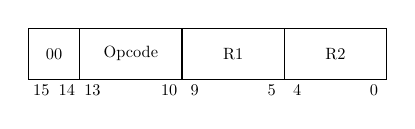
\begin{tikzpicture}[scale=.65, every node/.style={scale=0.59}]
  \draw (0,0) rectangle (7,1);
  \foreach \x in {1,3,5} \draw (\x,0) -- (\x,1);
  \node at (0.5,0.5) {00};
  \node at (2,0.5) {Opcode};
  \node at (4,0.5) {R1};
  \node at (6,0.5) {R2};

  \node[below] at (0.25,0) {15};
  \node[below] at (0.75,0) {14};
  \node[below] at (1.25,0) {13};
  \node[below] at (2.75,0) {10};
  \node[below] at (3.25,0) {9};
  \node[below] at (4.75,0) {5};
  \node[below] at (5.25,0) {4};
  \node[below] at (6.75,0) {0};
\end{tikzpicture}

\subsection*{32-bit Immediate Format}
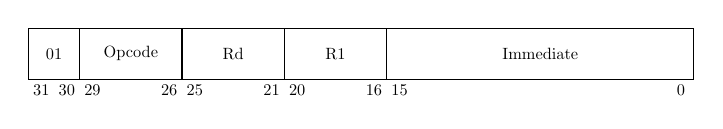
\begin{tikzpicture}[scale=.65, every node/.style={scale=0.59}]
  \draw (0,0) rectangle (13,1);
  \foreach \x in {1,3,5,7} \draw (\x,0) -- (\x,1);
  \node at (0.5,0.5) {01};
  \node at (2,0.5) {Opcode};
  \node at (4,0.5) {Rd};
  \node at (6,0.5) {R1};
  \node at (10,0.5) {Immediate};

  \node[below] at (0.25,0) {31};
  \node[below] at (0.75,0) {30};
  \node[below] at (1.25,0) {29};
  \node[below] at (2.75,0) {26};
  \node[below] at (3.25,0) {25};
  \node[below] at (4.75,0) {21};
  \node[below] at (5.25,0) {20};
  \node[below] at (6.75,0) {16};
  \node[below] at (7.25,0) {15};
  \node[below] at (12.75,0) {0};
\end{tikzpicture}

%Length[31:30] | Opcode[29:26] | RD[25:21] | R1[20:16] | R2[15:11] | Family[10:9] | Func[8:0]

\subsection*{32-bit Register Format}
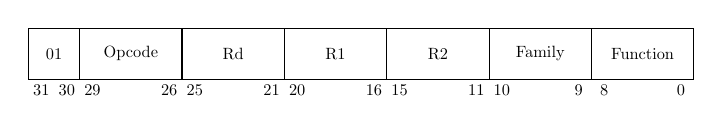
\begin{tikzpicture}[scale=.65, every node/.style={scale=0.59}]
  \draw (0,0) rectangle (13,1);
  \foreach \x in {1,3,5,7,9,11} \draw (\x,0) -- (\x,1);
  \node at (0.5,0.5) {01};
  \node at (2,0.5) {Opcode};
  \node at (4,0.5) {Rd};
  \node at (6,0.5) {R1};
  \node at (8,0.5) {R2};
  \node at (10,0.5) {Family};
  \node at (12,0.5) {Function};

  \node[below] at (0.25,0) {31};
  \node[below] at (0.75,0) {30};
  \node[below] at (1.25,0) {29};
  \node[below] at (2.75,0) {26};
  \node[below] at (3.25,0) {25};
  \node[below] at (4.75,0) {21};
  \node[below] at (5.25,0) {20};
  \node[below] at (6.75,0) {16};
  \node[below] at (7.25,0) {15};
  \node[below] at (8.75,0) {11};
  \node[below] at (9.25,0) {10};
  \node[below] at (10.75,0) {9};
  \node[below] at (11.25,0) {8};
  \node[below] at (12.75,0) {0};
\end{tikzpicture}

\subsection*{32-bit Register Format: Mult/Div}
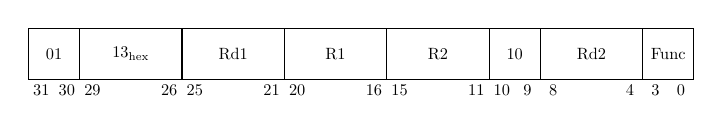
\begin{tikzpicture}[scale=.65, every node/.style={scale=0.59}]
  \draw (0,0) rectangle (13,1);
  \foreach \x in {1,3,5,7,9,10,12} \draw (\x,0) -- (\x,1);
  \node at (0.5,0.5) {01};
  \node at (2,0.5) {13$_{\text{hex}}$};
  \node at (4,0.5) {Rd1};
  \node at (6,0.5) {R1};
  \node at (8,0.5) {R2};
  \node at (9.5,0.5) {10};
  \node at (11,0.5) {Rd2};
  \node at (12.5,0.5) {Func};

  \node[below] at (0.25,0) {31};
  \node[below] at (0.75,0) {30};
  \node[below] at (1.25,0) {29};
  \node[below] at (2.75,0) {26};
  \node[below] at (3.25,0) {25};
  \node[below] at (4.75,0) {21};
  \node[below] at (5.25,0) {20};
  \node[below] at (6.75,0) {16};
  \node[below] at (7.25,0) {15};
  \node[below] at (8.75,0) {11};
  \node[below] at (9.25,0) {10};
  \node[below] at (9.75,0) {9};
  \node[below] at (10.25,0) {8};
  \node[below] at (11.75,0) {4};
  \node[below] at (12.25,0) {3};
  \node[below] at (12.75,0) {0};
\end{tikzpicture}

\subsection*{Format Abbreviations}
\begin{tabular}{lc}
\toprule
Format & Abbreviation \\
\midrule
16-bit & R1 \\
32-bit Immediate & I \\
32-bit Register & R2 \\
Pseudoinstruction & P \\
\bottomrule
\end{tabular}

\section*{Register Name, Number, and Use}
\begin{tabular}{ccl}
\toprule
Name & Number & Use \\
\midrule
Z & 0 & Fixed Constant 0 \\
A & 1 & Assembler Temporary \\
R2-R30 & 2-30 & General Purpose Registers \\
RA & 31 & Return Address \\
\bottomrule
\end{tabular}

\section*{Flags}
\begin{tabular}{cll}
\toprule
Code & Meaning & Setting Insts\\
\midrule
Z & Zero & Add/Sub/Cmp\\
C & Carry & Add/Sub/Cmp\\
N & Negative (sign bit) & Add/Sub/Cmp\\
O & Overflow & Add/Sub/Cmp/Mult/Div\\
D & Division by Zero & Div\\
\bottomrule
\end{tabular}

\section*{Branch to Flag}
\begin{tabular}{ll}
\toprule
Branch & Flag Check\\
\midrule
Equal & Z=1 \\
Not Equal & Z=0 \\
Greater Than & Z=0 and N=O \\
Greater Than or Equal & N=O \\
Greater Than Unsigned &  Z=0 and C=1\\
Greater Than or Equal Unsigned &  C=1\\
\bottomrule
\end{tabular}

\section*{Short Forms in Instruction Set}
\begin{tabular}{ll}
\toprule
Short Form & Description\\
\midrule
PC & Program Counter\\
Imm & Immediate\\
SignExtImm & \{16\{Immediate[15]\}, Immediate\} \\
ZeroExtImm & \{16'b0, Immediate\} \\
JMPAddr & \{PC[31:17], Immediate, 1'b0\} \\
NextInst & PC for next instruction \\
OpX & Imm, M[Reg], M[Reg + Imm] or R[Reg]\\
\bottomrule
\end{tabular}

\section*{Memory Format}
\begin{tabular}{ll}
\toprule
Format Rule & Setting\\
\midrule
Endianness & Little Endian\\
Bit Alignment & None\\
\bottomrule
\end{tabular}


\end{multicols}

\pagebreak

% Instruction set
\section*{Instruction Set}
\subsection*{Load/Store}
\begin{tabular}{>{\raggedright\arraybackslash\hangindent=0.5cm\hangafter=1}p{3cm}lc>{\raggedright\arraybackslash\hangindent=1.5cm\hangafter=1}p{5cm}lc}
\toprule
Instruction & Mnemonic & Format & Operation (in Verilog) & Assembly & Opcode(hex) \\
\midrule
Load Immediate & LDM & I & R[Rd] = SignExtImm & LDM Rd, Imm & 0\\
Load Immediate Upper & LDMU & I & R[Rd] = Immediate $<<$ 16 & LDMU Rd, Imm & 1\\
Load Word Direct & LDW(D) & I & R[Rd] = M[R1] & LDW Rd, [R1] & 2\\
Load Word Indexed & LDW(X) & I & R[Rd] = M[R1 + SignExtImm] & LDW Rd, Imm[R1] & 2\\
Load Half-Word Direct & LDH(D) & I & R[Rd] = \{16'b0, M[R1](15:0)\} & LDH Rd, [R1] & 3\\
Load Half-Word Indexed & LDH(X) & I & R[Rd] = \{16'b0, M[R1 + SignExtImm](15:0)\} & LDH Rd, Imm[R1] & 3\\
Load Byte Direct & LDB(D) & I & R[Rd] = \{24'b0, M[R1](7:0)\} & LDB Rd, [R1] & 4\\
Load Byte Indexed & LDB(X) & I & R[Rd] = \{24'b0, M[R1 + SignExtImm](7:0)\} & LDB Rd, Imm[R1] & 4\\
Store Word Direct & STW(D) & I & M[R1] = R[Rd]& STW Rd, [R1] & 5\\
Store Word Indexed & STW(X) & I & M[R1 + SignExtImm] = R[Rd] & STW Rd, Imm[R1] & 5\\
Store Half-Word Direct & STH(D) & I & M[R1] = R[Rd](15:0) & STH Rd, [R1] & 6\\
Store Half-Word Indexed & STH(X) & I & M[R1 + SignExtImm] = R[Rd](15:0) & STH Rd, Imm[R1] & 6\\
Store Byte Direct & STB(D) & I & M[R1] = R[Rd](7:0) & STB Rd, [R1] & 7\\
Store Byte Indexed & STB(X) & I & M[R1 + SignExtImm] = R[Rd](7:0) & STB Rd, Imm[R1] & 7\\
Load Jump Address & LDJ & I & R[Rd] = JMPAddr & LDJ Rd, Imm & 12\\
\bottomrule
\end{tabular}

 

\subsection*{Integer ALU}
\begin{tabular}{>{\raggedright\arraybackslash\hangindent=0.2cm\hangafter=1}p{2.5cm}lc>{\raggedright\arraybackslash\hangindent=2.5cm\hangafter=1}p{5cm}l>{\centering\arraybackslash}p{2cm}}
\toprule
Instruction & Mnemonic & Format & Operation (in Verilog) & Assembly & Opcode/Family/ Func(hex) \\
\midrule
Add Immediate & ADD(M) & P & R[Rd] = R[R1] + SignExtImm & ADD Rd, R1, Imm & --\\
Add Direct & ADD(D) & R2 & R[Rd] = R[R1] + M[R2] & ADD Rd, R1, [R2] & 13/0/0\\
Add Indexed & ADD(X) & P & R[Rd] = R[R1] + M[R2 + SignExtImm] & ADD Rd, R1, Imm[R2] & --\\
Add Register (destructive) & ADD(R) & R1 & R[R1] = R[R1] + R[R2] & ADD R1, R2 & 8\\
Add Register (non-destructive) & ADD(R) & R2 & R[Rd] = R[R1] + R[R2] & ADD Rd, R1, R2 & 13/0/1\\
Add PC & ADDPC & R2 & R[Rd] = PC + R[R1] & ADDPC Rd, R1 & 13/3/3\\
Subtract Immediate & SUB(M) & P & R[Rd] = R[R1] - SignExtImm & SUB Rd, R1, Imm & --\\
Subtract Direct & SUB(D) & R2 & R[Rd] = R[R1] - M[R2] & SUB Rd, R1, [R2] & 13/0/2\\
Subtract Indexed & SUB(X) & P & R[Rd] = R[R1] - M[R2 + SignExtImm] & SUB Rd, R1, Imm[R2] & --\\
Subtract Register (destructive) & SUB(R) & R1 & R[R1] = R[R1] - R[R2] & SUB R1, R2 & 9\\
Subtract Register (non-destructive) & SUB(R) & R2 & R[Rd] = R[R1] - R[R2] & SUB Rd, R1, R2 & 13/0/3\\
\bottomrule
\end{tabular}

\subsection*{Shift and Logical}
\begin{tabular}{>{\raggedright\arraybackslash\hangindent=0.2cm\hangafter=1}p{2.5cm}lc>{\raggedright\arraybackslash\hangindent=2.5cm\hangafter=1}p{5cm}l>{\centering\arraybackslash}p{2cm}}
\toprule
Instruction & Mnemonic & Format & Operation (in Verilog) & Assembly & Opcode/Family/ Func(hex) \\
\midrule
Not Register & NOT & R1 & R[R1] = $~\sim$R[R2] & NOT R1, R2 & 7 \\
And Immediate & AND(M) & P & R[Rd] = R[R1] \& ZeroExtImm & AND Rd, R1, Imm & --\\
And Direct & AND(D) & R2 & R[Rd] = R[R1] \& M[R2] & AND Rd, R1, [R2] & 13/1/0\\
And Indexed & AND(X) & P & R[Rd] = R[R1] \& M[R2 + ZeroExtImm] & AND Rd, R1, Imm[R2] & --\\
And Register & AND(R) & R2 & R[Rd] = R[R1] \& R[R2] & AND Rd, R1, R2 & 13/1/1\\
Or Immediate & OR(M) & I & R[Rd] = R[R1] \textbar ~ZeroExtImm & OR Rd, R1, Imm & 8\\
Or Direct & OR(D) & R2 & R[Rd] = R[R1] \textbar ~M[R2] & OR Rd, R1, [R2] & 13/1/2\\
Or Indexed & OR(X) & P & R[Rd] = R[R1] \textbar ~M[R2 + ZeroExtImm] & OR Rd, R1, Imm[R2] & --\\
Or Register & OR(R) & R2 & R[Rd] = R[R1] \textbar ~R[R2] & OR Rd, R1, R2 & 13/1/3\\
Xor Immediate & XOR(M) & P & R[Rd] = R[R1] $\oplus$ ZeroExtImm & XOR Rd, R1, Imm & --\\
Xor Direct & XOR(D) & R2 & R[Rd] = R[R1] $\oplus$ M[R2] & XOR Rd, R1, [R2] & 13/1/4\\
Xor Indexed & XOR(X) & P & R[Rd] = R[R1] $\oplus$ M[R2 + ZeroExtImm] & XOR Rd, R1, Imm[R2] & --\\
Xor Register & XOR(R) & R2 & R[Rd] = R[R1] $\oplus$ R[R2] & XOR Rd, R1, R2 & 13/1/5\\
Arithmetic Shift Right Immediate & ASR & R2 & R[Rd] = R[R1] $>>>$ R2 & ASR Rd, R1, R2 & 13/1/6\\
Arithmetic Shift Right Register & ASRR & R2 & R[Rd] = R[R1] $>>>$ R[R2] & ASRR Rd, R1, R2 & 13/1/7\\
Logical Shift Left Immediate & LSL & R2 & R[Rd] = R[R1] $<<$ R2 & LSL Rd, R1, R2 & 13/1/8\\
Logical Shift Left Register & LSLR & R2 & R[Rd] = R[R1] $<<$ R[R2] & LSLR Rd, R1, R2 & 13/1/9\\
Logical Shift Right Immediate & LSR & R2 & R[Rd] = R[R1] $>>$ R2 & LSR Rd, R1, R2 & 13/1/10\\
Logical Shift Right Register & LSRR & R2 & R[Rd] = R[R1] $>>$ R[R2] & LSRR Rd, R1, R2 & 13/1/11\\
Circular Shift Left Immediate & CSL & R2 & R[Rd] = \{R[R1], R[R1]\} $>>$ (32 - R2) & CSL Rd, R1, R2 & 13/1/12\\
Circular Shift Left Register & CSLR & R2 & R[Rd] =\{R[R1], R[R1]\} $>>$ (32 - R[R2]) & CSLR Rd, R1, R2 & 13/1/13\\
Circular Shift Right Immediate & CSR & R2 & R[Rd] = \{R[R1], R[R1]\} $>>$ R2 & CSR Rd, R1, R2 & 13/1/14\\
Circular Shift Right Register & CSRR & R2 & R[Rd] = \{R[R1], R[R1]\} $>>$ R[R2] & CSRR Rd, R1, R2 & 13/1/15\\
\bottomrule
\end{tabular}

\pagebreak

\subsection*{Multiply/Divide}
\begin{tabular}{>{\raggedright\arraybackslash\hangindent=0.5cm\hangafter=1}p{2.5cm}lc>{\raggedright\arraybackslash\hangindent=2cm\hangafter=1}p{5.5cm}>{\raggedright\arraybackslash\hangindent=1.5cm\hangafter=1}p{3.6cm}c}
\toprule
Instruction & Mnemonic & Format & Operation (in Verilog) & Assembly & Func(hex) \\
\midrule
Multiply Immediate & MULT(M) & P & \{R[Rd2], R[Rd1]\} = R[R1] * SignExtImm & MULT Rd1, Rd2, R1, Imm & --\\
Multiply Direct & MULT(D) & R2 & \{R[Rd2], R[Rd1]\} = R[R1] * M[R2] & MULT Rd, R1, [R2] & 0\\
Multiply Indexed & MULT(X) & P & \{R[Rd2], R[Rd1]\} = R[R1] * M[R2 + SignExtImm] & MULT Rd1, Rd2, R1, Imm[R2] & --\\
Multiply Register & MULT(R) & R2 & \{R[Rd2], R[Rd1]\} = R[R1] * R[R2] & MULT Rd1, Rd2, R1, R2 & 1\\
Multiply Immediate Unsigned & MULT(M)U & P & \{R[Rd2], R[Rd1]\} = R[R1] * ZeroExtImm & MULTU Rd1, Rd2, R1, Imm & --\\
Multiply Direct Unsigned & MULT(D)U & R2 & \{R[Rd2], R[Rd1]\} = R[R1] * M[R2] & MULTU Rd1, Rd2, R1, [R2] & 2\\
Multiply Indexed Unsigned & MULT(X)U & P & \{R[Rd2], R[Rd1]\} = R[R1] * M[R2 + SignExtImm] & MULTU Rd1, Rd2, R1, Imm[R2] & --\\
Multiply Register Unsigned & MULT(R)U & R2 & \{R[Rd2], R[Rd1]\} = R[R1] * R[R2] & MULTU Rd1, Rd2, R1, R2 & 3\\
Divide Immediate & DIV(M) & P & R[Rd1] = R[R1] / SignExtImm & DIV Rd1, Rd2, R1, Imm & --\\
&&&R[Rd2] = R[R1] \% SignExtImm\\
Divide Direct & DIV(D) & R2 & R[Rd1] = R[R1] / M[R2] & DIV Rd1, Rd2, R1, [R2] & 4\\
&&&R[Rd2] = R[R1] \% M[R2]\\
Divide Indexed & DIV(X) & P & R[Rd1] = R[R1] / M[R2 + SignExtImm] & DIV Rd1, Rd2, R1, Imm[R2] & --\\
&&&R[Rd2] = R[R1] \% M[R2 + SignExtImm]\\
Divide Register & DIV(R) & R2 & R[Rd1] = R[R1] / R[R2] & DIV Rd1, Rd2, R1, R2 & 5\\
&&&R[Rd2] = R[R1] \% R[R2]\\
Divide Immediate Unsigned & DIV(M)U & P & R[Rd1] = R[R1] / ZeroExtImm & DIVU Rd1, Rd2, R1, Imm & --\\
&&&R[Rd2] = R[R1] \% ZeroExtImm\\
Divide Direct Unsigned & DIV(D)U & R2 & R[Rd1] = R[R1] / M[R2] & DIVU Rd1, Rd2, R1, [R2] & 6\\
&&&R[Rd2] = R[R1] \% M[R2]\\
Divide Indexed Unsigned & DIV(X)U & P & R[Rd1] = R[R1] / M[R2 + SignExtImm] & DIVU Rd1, Rd2, R1, Imm[R2] & --\\
&&&R[Rd2] = R[R1] \% M[R2 + SignExtImm]\\
Divide Register Unsigned & DIV(R)U & R2 & R[Rd1] = R[R1] / R[R2] & DIVU Rd1, Rd2, R1, R2 & 7\\
&&&R[Rd2] = R[R1] \% R[R2]\\
Mult Low Half & MULT & P & R[Rd] = [R[R1] * Op2](31:0) & MULT Rd, R1, Op2 & --\\
Mult High Half & MULTH & P & R[Rd] = [R[R1] * Op2](63:32) & MULTH Rd, R1, Op2 & --\\
Mult Low Half Unsigned & MULTU & P &R[Rd] = [R[R1] * U(Op2)](31:0) & MULTU Rd, R1, Op2 & --\\
Mult High Half Unsigned & MULTHU & P & R[Rd] = [R[R1] * U(Op2)](63:32) & MULTHU Rd, R1, Op2 & --\\
Div Quotient & DIV & P & R[Rd] = R[R1] / Op2 & DIV Rd, R1, Op2 & --\\
Div Remainder & DIVR & P & R[Rd] = R[R1] \% Op2 & DIVR Rd, R1, Op2 & --\\
Div Quotient Unsigned & DIVU & P & R[Rd] = R[R1] / U(Op2) & DIVU Rd, R1, Op2 & --\\
Div Remainder Unsigned & DIVRU & P & R[Rd] = R[R1] \% U(Op2) & DIVRU Rd, R1, Op2 & --\\
\bottomrule
\end{tabular}

 

\subsection*{Branch}
\begin{tabular}{>{\raggedright\arraybackslash\hangindent=0.2cm\hangafter=1}p{2.5cm}lc>{\raggedright\arraybackslash\hangindent=2.5cm\hangafter=1}p{5.7cm}l>{\centering\arraybackslash}p{2cm}}
\toprule
Instruction & Mnemonic & Format & Operation (in Verilog) & Assembly & Opcode/Family/ Func(hex) \\
\midrule
Compare Immediate & CMP & P & SetFlags(R[R1] - SignExtImm) & CMP R1, Imm & --\\
Compare Direct & CMD & R2 & SetFlags(R[R1] - M[R2]) & CMP R1, [R2] & 13/3/2\\
Compare Indexed & CMX & P & SetFlags(R[R1] - M[R2 + SignExtImm]) & CMP R1, Imm[R2] & --\\
Compare Register & CMPR & R1 & SetFlags(R[R1] - R[R2]) & CMP R1, R2 & 6\\
Jump & JMP & P & PC = JMPAddr & JMP Immediate & --\\
Jump Register & JMPR & R1 & PC = R[R1] & JMPR R1 & 10\\
Jump and Link & JAL & P & PC = JMPAddr; R[RA] = NextInst & JAL Immediate & --\\
Jump and Link Register & JAL(R) & P & PC = JMPAddr; R[R1] = NextInst & JAL R1, Imm & --\\
Jump Register and Link & J(R)AL & P & PC = R[R1]; R[RA] = NextInst & JAL R1 & 11\\
Jump Register and Link Register & J(R)AL(R) & R1 & PC = R[R1]; R[R2] = PC + 2 & JAL R1, R2 & 11\\
Jump if Not Equal & JPN & I & If Flags, PC = PC + 4 + (SignExtImm $<<$ 1) & JPN Immediate & 9\\
Jump if Not Equal Register & JPN(R) & R1 & If Flags, PC = R[R1] & JPN R1 & 12\\
Jump if Equal & JPE & I & If Flags, PC = PC + 4 + (SignExtImm $<<$ 1) & JPE Immediate & 10\\
Jump if Equal Register & JPE(R) & R1 & If Flags, PC = R[R1] & JPE R1 & 13\\
Jump if Greater Than & JGT & I & If Flags, PC = PC + 4 + (SignExtImm $<<$ 1) & JGT Immediate & 11\\
Jump if Greater Than Register & JGT(R) & R1 & If Flags, PC = R[R1] & JGT R1 & 14\\
Jump if Greater Than Unsigned & JGTU & P & If Flags, PC = PC + 4 + (SignExtImm $<<$ 1) & JGTU Immediate & --\\
Jump if Greater Than Register Unsigned & JGT(R)U & R2 & If Flags, PC = R[R1] & JGTU R1 & 13/3/0\\
Jump if Greater Than or Equal & JGE & P & If Flags, PC = NextInst + (SignExtImm $<<$ 1) & JGE Immediate & --\\
Jump if Greater Than or Equal Register & JGE(R) & R1 & If Flags, PC = R[R1] & JGE R1 & 15\\
Jump if Greater Than or Equal Unsigned & JGEU & P & If Flags, PC = PC + 4 + (SignExtImm $<<$ 1) & JGEU Immediate & --\\
Jump if Greater Than or Equal Register Unsigned & JGE(R)U & R2 & If Flags, PC = R[R1] & JGEU R1 & 13/3/1\\
\bottomrule
\end{tabular}

 

\subsection*{Additional}
\begin{tabular}{>{\raggedright\arraybackslash\hangindent=0.2cm\hangafter=1}p{2.5cm}lc>{\raggedright\arraybackslash}p{5cm}lc}
\toprule
Instruction & Mnemonic & Format & Operation (in Verilog) & Assembly & Opcode/(hex) \\
\midrule
No Operation & NOOP & R1 & -- & NOOP & 0\\
End Program & END & R1 & PC = PC & END & 1\\
Increment & INC & R1 & R[R1] = R[R1] + 1 & INC R1 & 2\\
Decrement & DEC & R1 & R[R1] = R[R1] - 1 & DEC R1 & 3\\
Move Register & MOV & R1 & R[R1] = R[R2] & MOV R1, R2 & 4\\
Swap Registers & SWAPR & R1 & temp = R[R2]; R[R2] = R[R1]; R[R1] = temp & SWAPR R1, R2 & 5\\
\bottomrule
\end{tabular}
\end{document}
